

%\setcounter{chapter}{0}
\renewcommand{\theequation}{\thechapter.\arabic{equation}}
\numberwithin{equation}{chapter}
\baselineskip=8mm
\chapter{การวิเคราะห์เวกเตอร์}

\renewcommand{\thesection}{\thechapter.\arabic{section}}
\renewcommand{\theequation}{\thesection.\arabic{equation}}
\numberwithin{equation}{section}


%\section*{จุดประสงค์}
%\addtocontents{toc}{จุดประสงค์}

%\begin{enumerate}
%\renewcommand{\theenumi}{\roman{enumi}}
%\renewcommand{\labelenumi}{(\theenumi)}
%\item   สามารถอธิบายคุณสมบัติของปริมาณสเกลาร์และปริมาณเวกเตอร์ได้ และสามารถบอกความแตกต่างของปริมาณทั้งสองได้
%\item   สามารถบอกและแยกได้ว่า ปริมาณต่างๆ ทางฟิสิกส์ปริมาณใดเป็นปริมาณสเกลาร์และปริมาณใดเป็นปริมาณเวกเตอร์
%\item   สามารถบอกความหมายของเวกเตอร์หนึ่งหน่วย และหาเวกเตอร์หนึ่งหน่วยของเวกเตอร์ใดๆ ได้
%\item   สามารถแยกองค์ประกอบของเวกเตอร์ให้อยู่ในแนวแกนของพิกัดตั้งฉาก ทั้งในระบบ 2 มิติ และ 3 มิติ
%\item   สามารถรวมเวกเตอร์ตั้งแต่ 2 เวกเตอร์ขึ้นไปได้ โดยการใช้วิธีแยกองค์ประกอบของเวกเตอร์ให้อยู่ในแต่ละแกนของพิกัดตั้งฉาก แล้วรวมเวกเตอร์ลัพธ์จากแต่ละแกน
%\item   สามารถรวมเวกเตอร์ 2 เวกเตอร์ได้ โดยการใช้สมการการรวมเวกเตอร์และได้ขนาดของเวกเตอร์ลัพธ์ $\vec{C}$ จากการรวมเวกเตอร์ $\vec{A}$ และ $\vec{B}$ ได้จากสมการ $C=\sqrt{A^2+B^2+2AB\cos\theta}$ และหามุมของเวกเตอร์ลัพธ์ได้จาก $\alpha =\tan^{-1}\left(\frac{B\sin\theta}{A+B\cos\theta}\right)$ เมื่อเทียบกับเวกเตอร์ $\vec{A}$ หรือจากการใช้สมการกฎของโคไซน์
%\item   สามารถหาผลคูณสเกลาร์ของเวกเตอร์ 2 เวกเตอร์ และหาปริมาณที่เกี่ยวข้องกับการคูณสเกลาณ์ได้ เช่น มุมระหว่างเวกเตอร์ทั้งสอง หรือหาเวกเตอร์อีกเวกเตอร์หนึ่งเมื่อทราบค่ามุม
%\item   สามารถหาผลคูณเวกเตอร์ของเวกเตอร์ 2 เวกเตอร์ และหาปริมาณที่เกี่ยวข้องกับการคูณเวกเตอร์ได้ เช่น พื้นที่
%\end{enumerate}








%\section{บทนำ}
%\noindent
โดยทั่วไปในทางฟิสิกส์ คณิตศาสตร์ได้ถือว่าเป็นเครื่องมือที่ช่วยให้นักฟิสิกส์สามารถทำความเข้าใจกับปรากฏการณ์ทางธรรมชาติได้มากยิ่งขึ้น โดยเริ่มตั้งแต่คณิตศาสตร์พื้นฐาน ตัวอย่างเช่น การดำเนินการทาง สเกลาร์ (scalar), เวกเตอร์ (vector) และเทนเซอร์ (tensor) ไม่ว่าจะเป็น เกรเดียน (gradient), ไดเวอร์เจนซ์ (divergence) หรือ เคิร์ล (curl) จนกระทั่งการดำเนินการขั้นสูง ตัวอย่างเช่น การหาอนุพันธ์ การอินทิเกรต สมการเชิงอนุพันธ์ หรือแม้แต่การนำฟังก์ชันทางคณิตศาสตร์มาประยุกต์ใช้ในฟิสิกส์ ตัวอย่างเช่น สมการเลอจองด์ (Legendre Equation) สมการพัวซองค์ (Poisson's Equation) ที่เอาไปประยุกต์ใช้กับวิชาฟิสิกส์ขั้นสูง อย่างวิชากลศาสตร์ควอนตัม (Quantum Mechanics) เป็นต้น \cite{Edmund:Dynamics, Planck 2015, wmap9}

สำหรับเนื้อหาในบทนี้ จะแนะนำให้รู้จักกับพื้นฐานเกี่ยวกับปริมาณทางฟิสิกส์ ได้แก สเกลาร์, เวกเตอร์ และเทนเซอร์เบื้องต้น ในระบบพิกัดฉาก (Cartesian Coordinate) รวมถึงการดำเนินการทางคณิตศาสตร์ นอกจากนี้ยังจะแนะนำเกี่ยวกับการแปลงระบบพิกัดจากระบบพิกัดฉาก ($x$, $y$, $z$) ไปเป็นระบบพิกัดทรงกระบอก (Circular Cylinder Coordinate) หรือไปเป็นระบบพิกัดแบบทรงกลม (Spherical Polar Coordinate) พร้อมทั้งการดำเนินการทางคณิตศาสตร์ในระบบพิกัดดังกล่าวเหล่านั้นด้วยเช่นกัน \cite{Power-law, intro:cosmology}

%-----------------------------------------------------------------
\section{การดำเนินการพื้นฐานเกี่ยวกับเวกเตอร์}

ในทางวิทยาศาสตร์ ปริมาณพื้นฐานทั่วไปจะแบ่งได้เป็น ปริมาณที่มีแต่ขนาด หรือบอกแค่ขนาดก็มีความหมายที่สมบูรณ์ ปริมาณนั้นเราเรียกว่า \textit{ปริมาณสเกลาร์} (scalar) เช่น เวลา อุณภูมิ ความยาว เป็นต้น นอกจากนี้ยังมีปริมาณที่ต้องบอกทั้งขนาดและทิศทาง จึงจะมีความหมายสมบูรณ์ ปริมาณนั้นเรียกว่า \textit{ปริมาณเวกเตอร์} (vector) เช่น ความเร็ว ความเร่ง ระยะกระจัด เป็นต้น ซึ่งปริมาณพื้นฐานเหล่านี้สามารถดำเนินการทางคณิตศาสตร์หว่างกันได้

ถ้ามีเวกเตอร์ $\vec{A} = A_x\hat{i} + A_y\hat{j} + A_z\hat{k}$ และเวกเตอร์ $\vec{B} = B_x\hat{i} + B_y\hat{j} + B_z\hat{k}$ เมื่อ $ \i, \j, \k$ เป็นเวกเตอร์หน่วย (unit vector) ที่ชี้ไปในทิศทางตามแนวแกน $x$, $y$, และ $z$ ตามลำดับ แล้วเราสามารถหาขนาดของเวกเตอร์ $\vec{A}$ ได้จาก
\begin{equation}\label{MagA}
|\vec{A}| = \sqrt{A_x^2 + A_y^2 + A_z^2}
\end{equation}
และยังสามารถทำการบวกและลบเวกเตอร์ระหว่างสองเวกเตอร์ได้ดังนี้
\begin{equation}\label{ApmB}
\vec{A} \pm \vec{B} = (A_x + B_x)\i \pm (A_y + B_y)\j \pm (A_z + B_z)\k
\end{equation}
สำหรับการคูณเวกเตอร์นั้นมี 2 แบบ คือ การคูณแบบดอท (dot product) และการคูณแบบครอส (cross product) ดังนี้

\subsection{การคูณแบบดอท (Dot Product)}

เป็นการคูณของเวกเตอร์สองตัวที่ให้ผลลัพธ์เป็นปริมาณสเกลาร์ โดยเราสามารถเรียกอีกอย่างหนึ่งว่า การคูณแบบสเกลาร์ (scalar product) ก็ได้ ดังนี้
\begin{eqnarray}\label{AdotB}
\vec{A} \cdot \vec{B} &=& (A_x\hat{i} + A_y\hat{j} + A_z\hat{k})\cdot (B_x\hat{i} + B_y\hat{j} + B_z\hat{k}) \no \\
        &=& A_xB_x(\i\cdot\i) + A_xB_y(\i\cdot\j) + A_xB_z(\i\cdot\k) \no \\
        & & A_yB_x(\j\cdot\i) + A_yB_y(\j\cdot\j) + A_yB_z(\j\cdot\k) \no \\
        & & A_zB_x(\k\cdot\i) + A_zB_y(\k\cdot\j) + A_zB_z(\k\cdot\k) \no \\
        &=& A_xB_x + A_yB_y + A_zB_z
\end{eqnarray}
โดยในการนี้ เราใช้การหาขนาดของการคูณเวกเตอร์แบบดอท คือ
\begin{eqnarray}\label{AdotBangle}
|\vec{A}|\cdot|\vec{B}| &=& |\vec{A}||\vec{B}|\cos \theta \no \\
\vec{A}\cdot\vec{B} &=& AB\cos \theta
\end{eqnarray}
เมื่อ $\theta$ เป็นมุมที่เกิดขึ้นระหว่างเวกเตอร์ $\vec{A}$ และเวกเตอร์ $\vec{B}$ ดังรูปที่ \ref{fig1} และ $A = |\vec{A}|$, $B = |\vec{B}|$ เป็นขนาดของเวกเตอร์ $\vec{A}$ และเวกเตอร์ $\vec{B}$ ตามลำดับ ดังนั้นสำหรับเวกเตอร์หน่วย $\i, \j, \k$ แต่ละตัวจะมีขนาดเป็น 1 และมุมระหว่างเวกเตอร์หน่วยเดียวกันเป็น 0 องศา และมุมระหว่างเวกเตอร์หน่วยที่ต่างกันเป็น 90 องศา ทำให้ $\cos 0 = 1$ และ $\cos 90 = 0$ ดังนั้น สำหรับเวกเตอร์หน่วยที่ดอทกัน จะได้ว่า
\begin{equation}\label{eq:DotUnit}
  \begin{aligned}
    \i\cdot\i = \j\cdot\j = \k\cdot\k &= 1 \\
    \i\cdot\j = \i\cdot\k = \j\cdot\k &= 0
  \end{aligned}
\end{equation}
ดังนั้น เมื่อเรานำเวกเตอร์สองตัวมาดอทกันจึงได้ผลลัพธ์ดังแสดงในสมการ (\ref{AdotB}) หากการคูณแบบดอทนี้เป็นการคูณกันระหว่างเวกเตอร์ตัวเดียวกัน เราจะได้ว่า
\begin{equation}
\vec{A}\cdot\vec{A} = A^2 = A_x^2 + A_y^2 + A_z^2
\end{equation}
และขนาดของเวกเตอร์ $\vec{A} = A = \sqrt{A_x^2 + A_y^2 + A_z^2}$

\begin{figure}%[!h]%%Figure 1
\centering
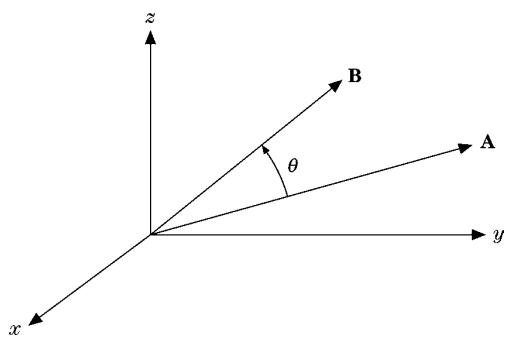
\includegraphics[width=0.5\columnwidth]{vector-01.png}
\caption{การคูณเวกเตอร์แบบดอท $\vec{A}\cdot\vec{B} = AB\cos \theta$ (ภาพจาก Arfken 2005)}
\label{fig1}
\end{figure}

\begin{figure}%[!h]%%Figure 2
\centering
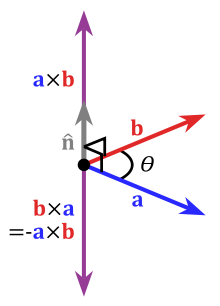
\includegraphics[width=0.5\columnwidth]{220px-Cross_product_vector.svg.png}
\caption{การคูณเวกเตอร์แบบครอส $\vec{A}\cross\vec{B} = AB\sin \theta$ (ภาพจากอินเตอร์เนต)}
\label{fig2}
\end{figure}

\subsection{การคูณแบบครอส (Cross Product)}

เป็นการคูณที่ให้ผลลัพธ์ออกมาเป็นปริมาณเวกเตอร์ และเวกเตอร์ใหม่ที่ได้นั้น ก็จะมีทิศตั้งฉากกับเวกเตอร์ทั้งสองที่นำมาครอสกัน หรือเราสามารถเรียกได้อีกอย่างว่า การคูณแบบเวกเตอร์ (vector product) ก็ได้ นั่นคือ
\begin{equation}\label{AcrossB}
\vec{A}\cross\vec{B} = \vec{C}
\end{equation}
เราจะได้ว่า $\vec{C}$ จะมีทิศทางตั้งฉากกับเวกเตอร์ $\vec{A}\cross\vec{B}$ ดังรูปที่ \ref{fig2} โดยขนาดของเวกเตอร์ $\vec{C} = C$ สามารถหาได้จาก
\begin{equation}\label{MagC}
|\vec{C}| = |\vec{A}\cross\vec{B}| = AB\sin \theta
\end{equation}
เมื่อ $\theta$ เป็นมุมระหว่างเวกเตอร์ $\vec{A}$ และเวกเตอร์ $\vec{B}$ นอกจากนี้ เรายังสามารถเขียนเวกเตอร์ $\vec{C}$ ได้ดังนี้
\begin{eqnarray}\label{vecC}
\vec{A}\cross\vec{B} &=& \vec{C} \no \\
        &=& (A_x\hat{i} + A_y\hat{j} + A_z\hat{k})\cross (B_x\hat{i} + B_y\hat{j} + B_z\hat{k}) \no \\
        &=& A_xB_x(\i\cross\i) + A_xB_y(\i\cross\j) + A_xB_z(\i\cross\k) \no \\
        & & A_yB_x(\j\cross\i) + A_yB_y(\j\cross\j) + A_yB_z(\j\cross\k) \no \\
        & & A_zB_x(\k\cross\i) + A_zB_y(\k\cross\j) + A_zB_z(\k\cross\k) \no \\
        &=& (A_yB_z - A_zB_y)\i + (A_zB_x - A_xB_z)\j \no \\
        & & +\;(A_xB_y - A_yB_x)\k
\end{eqnarray}
โดยอาศัยคุณลักษณะของการครอสของเวกเตอร์หน่วย ดังนี้
\begin{eqnarray}\label{eq:CrossUnit}
\i\cross\i = \j\cross\j = \k\cross\k &=& 0 \no \\
\i\cross\j = \k, \;\;\;\;\j\cross\k = \i, \;\;\;\;\k\cross\i &=& \j \\
\j\cross\i = - \k, \;\k\cross\j = - \i, \;\i\cross\k &=& - \j \no
\end{eqnarray}
ทำนองเดียวกัน หากเราทำการสลับตำแหน่งของเวกเตอร์ $\vec{A}\cross\vec{B}$ เราจะได้ว่า
\begin{equation}\label{BcrossA}
\vec{B}\cross\vec{A} = - \vec{A}\cross\vec{B}
\end{equation}
ผลลัพธ์ที่ได้จะเป็นเวกเตอร์ที่มีขนาดเท่ากับเวกเตอร์ผลลัพธ์ที่เกิดจากการคูณเวกเตอร์แบบครอส แต่จะมีทิศทางตรงกันข้าม ดังแสดงในรูปที่ \ref{fig2} ในทำนองเดียวกัน หากเป็นการคูณแบบครอสของเวกเตอร์เดียวกัน ผลลัพธ์ที่ได้จะเป็นเวกเตอร์ศูนย์ (zero vector)

การคูณเวกเตอร์แบบครอสยังสามารถใช้กระบวนการทางเมตริกซ์ (matrix) เพื่อหาผลคูณได้เช่นกัน โดยอาศัยการจัดเวกเตอร์ที่ครอสกันในรูปแบบของเมตริกซ์แล้วทำการหาดีเทอร์มิแนนท์ (determinant of matrix หรือ det) ซึ่งมีรูปแบบดัง
\begin{eqnarray}\label{AcrossBMatrix}
\vec{A}\cross\vec{B} &=& \begin{vmatrix} \i & \j & \k \\ A_x & A_y & A_z \\ B_x & B_y & B_z \end{vmatrix} \no \\
        &=& \begin{vmatrix}A_y & A_z \\ B_y & B_z \end{vmatrix}\i + \begin{vmatrix}A_x & A_z \\ B_x & B_z \end{vmatrix}\j + \begin{vmatrix}A_x & A_y \\ B_x & B_y \end{vmatrix}\k \no \\
        &=& (A_yB_z - A_zB_y)\i + (A_zB_x - A_xB_z)\j \no \\
        & & +\;(A_xB_y - A_yB_x)\k
\end{eqnarray}

\subsection{ผลคูณสามเวกเตอร์ (Triple Product)}

เป็นการคูณของเวกเตอร์สามตัว ซึ่งเราเรียกว่า \textit{ผลคูณสามเวกเตอร์} (triple product) ซี่งประกอบไปด้วย \\
\subsubsection{ผลคูณสามเวกเตอร์แบบสเกลาร์ (scalar triple product)}

เป็นการคูณที่มีทั้งการคูณแบบดอทและแบบครอสผสมกันอยู่ ซึ่งผลลัพธ์ที่ได้จะเป็นปริมาณสเกลาร์ ซึ่งสามารถเขียนได้ว่า $\vec{A}\cdot(\vec{B}\cross\vec{C}) = \vec{A}\cdot\vec{B}\cross\vec{C}$ โดยในการหาผลคูณต้องทำการหาผลคูณแบบครอสก่อนเสมอแล้วจึงทำการหาผลคูณแบบดอทเป็นลำดับสุดท้าย ดังนี้
\begin{eqnarray}\label{TripleScalarProd}
\vec{A}\cdot\vec{B}\cross\vec{C} &=& (A_x\hat{i} + A_y\hat{j} + A_z\hat{k})\cdot\Big[(B_yC_z - B_zC_y)\i + (B_zC_x - B_xC_z)\j \no \\
        & & +\;(B_xC_y - B_yC_x)\k\Big] \no \\
        &=& A_x(B_yC_z - B_zC_y) + A_y(B_zC_x - B_xC_z) \no \\
        & & +\;A_z(B_xC_y - B_yC_x)
\end{eqnarray}
และผลลัพธ์ที่ได้มีขนาดเท่ากับปริมาตรของทรงสี่เหลี่ยมด้านขนานที่มีเวกเตอร์ทั้งสามประกอบเป็นด้านทั้งสามของทรงสี่เหลี่ยมด้านขนาน ดังรูปที่ \ref{fig3} และการคูณแบบนี้ยังสามารถหาแบบเมตริกซ์ได้ ดังนี้
\begin{eqnarray}\label{ScalarTripleProdMatrix}
\vec{A}\cdot\vec{B}\cross\vec{C} &=& \begin{vmatrix} A_x & A_y & A_z \\ B_x & B_y & B_z \\ C_x & C_y & C_z \end{vmatrix} \no \\
        &=& A_x(B_yC_z - B_zC_y) + A_y(B_zC_x - B_xC_z) \no \\
        & & +\;A_z(B_xC_y - B_yC_x)
\end{eqnarray}
การคูณแบบนี้ยังมีคุณลักษณะพิเศษที่สามารถเรียงสลับกันได้ โดยผลคูณที่ได้ไม่เปลี่ยนแปลง ซึ่งเราเรียกลักษณะนี้ว่า \textit{การเรียงลำดับหมุนวน} (cyclic order permutation) และสามารถเขียนได้เป็น
\begin{equation}\label{ScalarTripleProdCyclicOrder}
\vec{A}\cdot\vec{B}\cross\vec{C} = \vec{B}\cdot\vec{C}\cross\vec{A} = \vec{C}\cdot\vec{A}\cross\vec{B}
\end{equation}
นอกจากนี้ก็จะมีคุณสมบัติ \textit{แอนไทคอมมิวท์} (anticommutativity) ดังนี้
\begin{equation}\label{ScalarTripleProdAntiCommute}
\vec{A}\cdot\vec{B}\cross\vec{C} = \begin{cases} - \vec{A}\cdot\vec{C}\cross\vec{B}  \\
                                                            - \vec{B}\cdot\vec{A}\cross\vec{C} \\
                                                            - \vec{C}\cdot\vec{B}\cross\vec{A} \end{cases}
\end{equation}

\begin{figure}%[!h]%%Figure 3
\centering
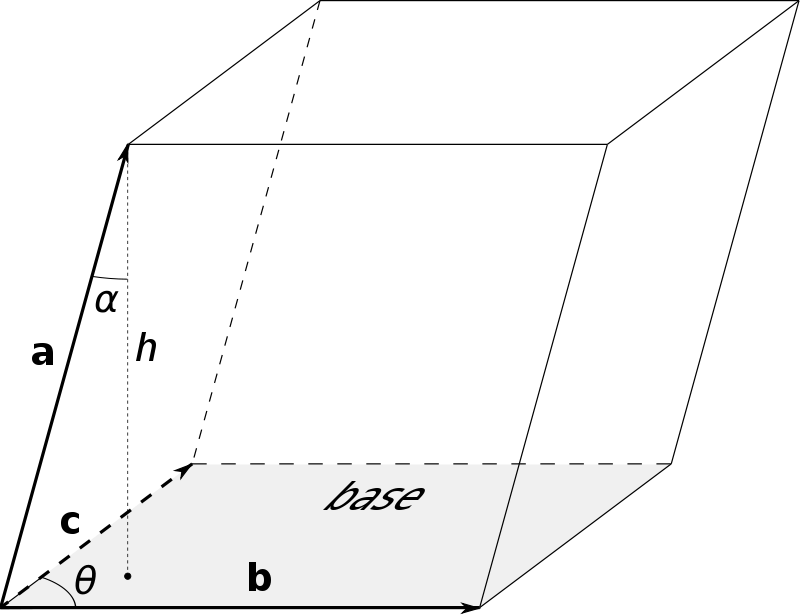
\includegraphics[width=0.8\columnwidth]{800px-Parallelepiped_volume.svg.png}
\caption{การคูณสามเวกเตอร์แบบสเกลาร์ $\vec{A}\cdot\vec{B}\cross\vec{C}$ ซึ่งผลลัพธ์ที่ได้จะมีขนาดเท่ากับปริมาตรของทรงสี่เหลี่ยมด้านขนาน (ภาพจากอินเตอร์เนต)}
\label{fig3}
\end{figure}

\subsubsection{การคูณสามเวกเตอร์แบบเวกเตอร์ (vector triple product)}

ในการคูณแบบนี้เราสามารถหาผลคูณได้จากสมการ
\begin{equation}\label{VectorTripleProd}
\vec{A}\cross\vec{B}\cross\vec{C} = \vec{B}(\vec{A}\cdot\vec{C}) - \vec{C}(\vec{A}\cdot\vec{B})
\end{equation}
การคูณแบบนี้เรียกว่า \textit{การกระจายผลคูณสามเวกเตอร์} (triple product expansion) หรือ \textit{สูตรลากรองจ์} (Lagrange's formula) ซึ่งมักจะมีการจำแบบง่ายๆว่า ``BAC ลบ CAB'' นอกจากนี้ยังมีสมบัติที่น่าสนใจ ดังนี้
\begin{itemize}
    \item แอนไทคอมมิวต์ (Anticommutivity)
        \begin{equation}\label{VectorTripleProdAntiCommute}
            (\vec{A}\cross\vec{B})\cross\vec{C} = - \vec{C}(\cross\vec{A}\cross\vec{B}) = - (\vec{C}\cdot\vec{B})\vec{A} + (\vec{C}\cdot\vec{A})\vec{B}
        \end{equation}
    \item คุณลักษณ์ของจาโคบี (Jacobi identity)
        \begin{equation}\label{VectorTripleProdJacobiIden}
            \vec{A}\cross(\vec{B}\cross\vec{C}) + \vec{B}\cross(\vec{C})\cross\vec{A}) + \vec{C}\cross(\vec{A})\cross\vec{B}) = 0
        \end{equation}
    \item สมการรูปแบบอื่นๆที่น่าสนใจ
        \begin{equation}\label{VectorTripleProdOthers}
            (\vec{A}\cross\vec{B})\cross\vec{C} = \vec{A}\cross(\vec{B}\cross\vec{C}) - \vec{B}\cross(\vec{A}\cross\vec{C})
        \end{equation}
\end{itemize}

\begin{center}
\Large{\textbf{แบบฝึกหัด}}\\
\end{center}
1. ถ้าเรามีเวกเตอร์ $\vec{C} = \vec{A} + \vec{B}$ จงพิสูจน์กฎของโคไซน์ (law of cosine) \\
$C^2 = A^2 + B^2 + 2AB\cos\theta$\\
2. พิจารณาเวกเตอร์ $\vec{A}$, $\vec{B}$, และ $\vec{C}$ ดังต่อไปนี้
\begin{eqnarray}\label{Excercise01}
\vec{A} &=& 3\i - 2\j + 2\k \no \\
\vec{B} &=& 6\i + 4\j - 2\k \no \\
\vec{C} &=& -3\i - 2\j - 4\k \no
\end{eqnarray}
จงคำนวณหาค่าของ $\vec{A}\cdot\vec{B}\cross\vec{C}$ และ $\vec{A}\cross\vec{B}\cross\vec{C}$

\section{การดำเนินการขั้นสูงกับเวกเตอร์}

การดำเนินการขั้นสูงกับเวกเตอร์นั้นประกอบไปด้วยการดำเนินการทั้งสิ้น 3 รูปแบบ คือ เกรเดียนท์ (gradient, $\nabla$), ไดเวอร์เจนซ์ (divergence, $\nabla\cdot$) และเคิร์ล (curl, $\nabla\cross$) ดังนี้

\subsection{เกรเดียนท์ (Gradient, $\nabla$)}

ถ้าเรามีสเกลาร์ฟังก์ชันใดๆ $F(x, y, z)$ แล้วเกรเดียนท์ของฟังก์ชัน $F(x, y, z)$ นี้สามารถเขียนได้เป็น $grad \;F(x, y, z)$ หรือ $\nabla F(x, y, z)$ และสามารถเขียนได้เป็น
\begin{eqnarray}\label{GradF}
grad \;F(x, y, z) &=& \nabla F(x, y, z) \no \\
        &=& \l(\pdx\i + \pdy\j + \pdz\k\r) F(x, y, z) \no \\
        &=& \f{\pd F(x, y, z)}{\pd x}\i + \f{\pd F(x, y, z)}{\pd y}\j + \f{\pd F(x, y, z)}{\pd z}\k
\end{eqnarray}
เมื่อ $grad$ (อ่านว่า แกรด) หรือ $\nabla$ (อ่านว่า เดล) เขียนได้เป็น
\begin{equation}\label{NablaDef}
\nabla = \pdx\i + \pdy\j + \pdz\k
\end{equation}
เกรเดียนท์มีคุณลักษณะเหมือนกันกับเวกเตอร์ทั่วไป คือ มีทั้งขนาดและทิศทาง โดยที่ \emph{เกรเดียนท์ $\nabla F$ จะมีทิศทางที่ชี้ไปยังทิศที่มีแนวโน้มที่เพิ่มขึ้นมากที่สุดของฟังก์ชัน $F$} และนอกจากนี้ \emph{ขนาดของเกรเดียนท์ $|\nabla F|$ จะเป็นค่าความชัน (ด้วยอัตราการเพิ่มขึ้น) ตามทิศทางที่ให้ค่าสูงสุดนั้น} เราสามารถจินตนาการว่าเรายืนอยู่ตีนเขา และเมื่อมองไปรอบๆ เราจะมองเห็นทางที่สูงขึ้นไปบนเขา ซึ่งนั้นก็คือ \emph{ทิศทาง}ของเกรเดียนท์ และเมื่อทำการวัดความชันในทิศทางนั้น (ขึ้นเขา) นั่นก็คือ \emph{ขนาด}ของเกรเดียนท์ นั่นเอง

\subsection{ไดเวอร์เจนซ์ (Divergence, $\nabla\cdot$)}

เป็นการดำเนินการแบบเวกเตอร์เมื่อมีเวกเตอร์ฟังก์ชัน $\vec{V} = V_x\i + V_y\j + V_z\k$ แล้วไดเวอร์เจนซ์ของเวกเตอร์ $\vec{V}$ สามารถเขียนได้เป็น
\begin{eqnarray}\label{DivV}
\nabla\cdot\vec{V} &=& div\;\vec{V} \no \\
        &=& \l(\pdx\i + \pdy\j + \pdz\k\r)\cdot\l(V_x\i + V_y\j + V_z\k\r) \no \\
        &=& \f{\pd V_x}{\pd x} + \f{\pd V_y}{\pd y} + \f{\pd V_z}{\pd z}
\end{eqnarray}
ผลลัพธ์ที่ได้จะเป็นปริมาณสเกลาร์ นอกจากนี้ ยังสามารถดำเนินการแบบผสม คือ มีสเกลาร์ฟังก์ชันกับเวกเตอร์ฟังก์ชันอยู่ด้วยกัน ซึ่งสามารถเขียนได้เป็น
\begin{equation}\label{DivFV}
\nabla\cdot(F\vec{V}) = (\nabla F)\cdot\vec{V} + F\nabla\cdot\vec{V}
\end{equation}
เมื่อ $F = F(x, y, z)$ เป็นสเกลาร์ฟังก์ชัน และถ้าไดเวอร์เจนซ์ของเวกเตอร์ฟังก์ชันใดเป็นศูนย์ คือ $\nabla\cdot\vec{B} = 0$ เราจะเรียกเวกเตอร์ฟังก์ชันนั้นว่าเป็นฟังก์ชันโซลีนอยด์ ซึ่งถ้าเมื่อเวกเตอร์ฟังก์ชันใดเป็นฟังก์ชันโซลีนอยด์ เวกเตอร์ฟังก์ชันนั้นสามารถเขียนในรูปของเคิร์ล (curl) ของเวกเตอร์อื่นได้ และเรียกเวกเตอร์อื่นใดนั้นว่าเป็นเวกเตอร์ศักย์ (vector potential)

ในการอธิบายเชิงกายภาพของไดเวอร์เจนซ์ เราจะพิจารณา $\nabla\cdot\vec{V}$ เป็นการวัดว่าเวกเตอร์ $\vec{V}$ จะพุ่งกระจาย (spreads out or diverges) จากจุดอ้างอิงได้มากน้อยเท่าไร จากรูปที่ \ref{fig4} ภาพ (a) จะเห็นว่ามีไดเวอร์เจนซ์บวกเพราะลูกศรพุ่งชี้ออกและมีขนาดเพิ่มขึ้น (ถ้าลูกศรพุ่งเข้าและมีขนาดลดลงเรื่อยๆ จะเรียกว่าเป็นไดเวอร์เจนซ์ลบ) ทำนองเดียวกันกับภาพ (c) ก็จะมีไดเวอร์เจนซ์บวก เช่นเดียวกันกับภาพ (a) ส่วนภาพ (b) ไม่มีไดเวอร์เจนซ์ หรือเรียกว่า ไดเวอร์เจนต์ศูนย์ (zero divergence)

\begin{figure}%[!h]%%Figure 4
\centering
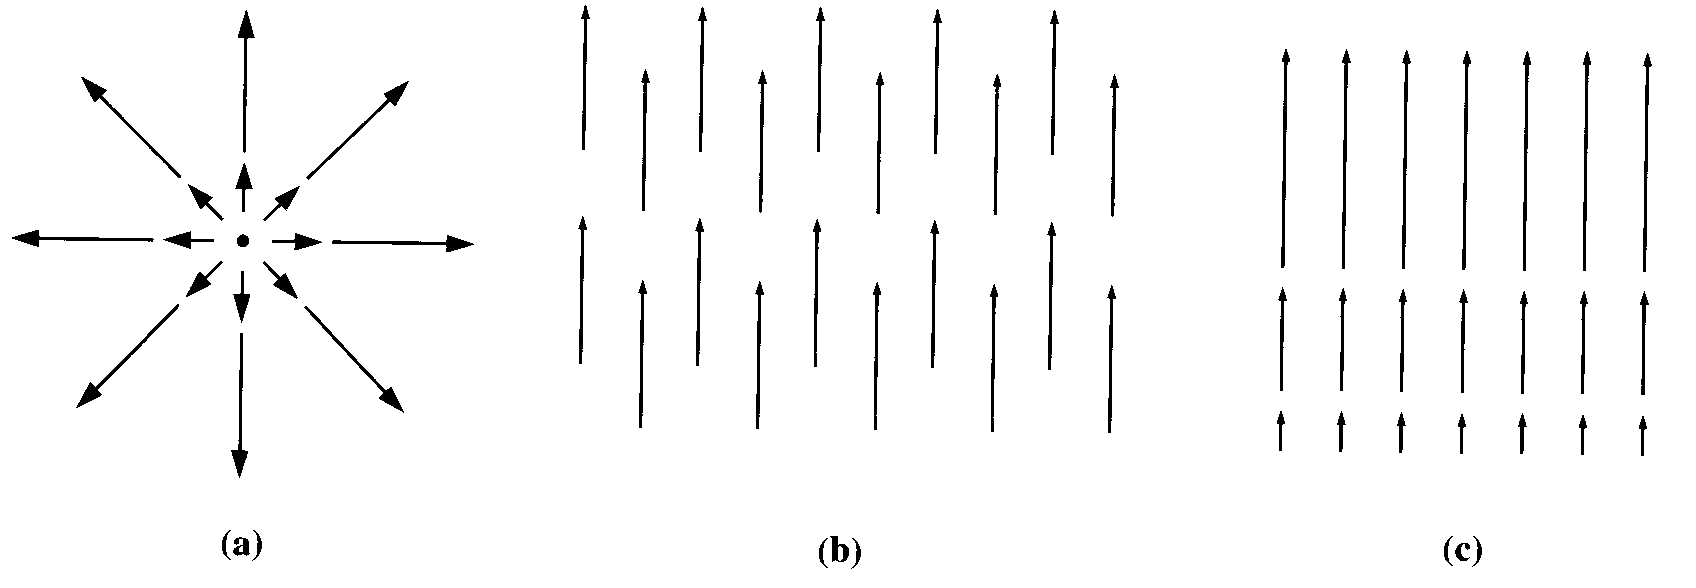
\includegraphics[width=1.0\columnwidth]{Divergence.png}
\caption{ไดเวอร์เจนซ์ $\nabla\cdot\vec{V}$ (a) มีไดเวอร์เจนซ์บวก (b) มีไดเวอร์เจนซ์ศูนย์ (c) มีไดเวอร์เจนซ์บวก (ภาพจาก Griffiths 1999)}
\label{fig4}
\end{figure}

ในกรณีของไดเวอร์เจนซ์เราสามารถเขียนไดเวอร์เจนซ์ซ้อนกับเกรเดียนท์ ได้เป็น
\begin{eqnarray}\label{LaplacianPsi}
\nabla\cdot\nabla\psi(x, y, z) &=& \nabla^2\psi \no \\
        &=& \f{\pd^2\psi}{\pd x^2} + \f{\pd^2\psi}{\pd y^2} + \f{\pd^2\psi}{\pd z^2}
\end{eqnarray}
โดย $\nabla^2$ อ่านว่า \emph{ลาปลาเซียน} (Laplacian)

\subsection{เคิร์ล (Curl, $\nabla\cross$)}

เป็นการดำเนินการแบบเวกเตอร์ ที่ให้ผลลัพธ์เป็นเวกเตอร์ สามารถเขียนได้เป็น
\begin{eqnarray}\label{CurlV}
\nabla\cross\vec{V} &=& curl\;\vec{V} \no \\
        &=& \l(\pdx\i + \pdy\j + \pdz\k\r)\cross\l(V_x\i + V_y\j + V_z\k\r) \no \\
        &=& \l(\pdy V_z - \pdz V_y\r)\i + \l(\pdz V_x - \pdx V_z\r)\j \no \\
         & & +\; \l(\pdx V_y - \pdy V_x\r)\k
\end{eqnarray}
หรือสามารถเขียนในรูปเมตริกซ์ได้เป็น
\begin{eqnarray}\label{CurlVMatrix}
\nabla\cross\vec{V} &=& \begin{vmatrix} \i & \j & \k \\ \pdx & \pdy & \pdz \\ V_x & V_y & V_z \end{vmatrix} \no \\
        &=& \l(\pdy V_z - \pdz V_y\r)\i + \l(\pdz V_x - \pdx V_z\r)\j \no \\
        & & +\; \l(\pdx V_y - \pdy V_x\r)\k
\end{eqnarray}
จะเห็นว่าได้ผลลัพธ์เช่นเดียวกันกับสมการที่ (\ref{CurlV}) และถ้ามีเคิร์ลของเวกเตอร์ $\vec{V}$ ใดๆเป็นศูนย์ นั่นคือ $\nabla\cross\vec{V} = 0$ เราจะเรียกเวกเตอร์ $\vec{V}$ นี้ว่า ไม่สามารถหมุนได้ (irrotational)

ในการอธิบายเชิงกายภาพของเคิร์ล เราจะพิจารณา $\nabla\cross\vec{V}$ เป็นการวัดปริมาณการหมุนวนของเวกเตอร์ $\vec{V}$ รอบจุดอ้างอิง ดังแสดงในรูปที่ \ref{fig5} จะเห็นว่ามีการหมุนวนรอบแกน $z$ ซึ่งเป็นทิศทางของ $\nabla\cross\vec{V}$ นั่นเอง

\begin{figure}%[!h]%%Figure 5
\centering
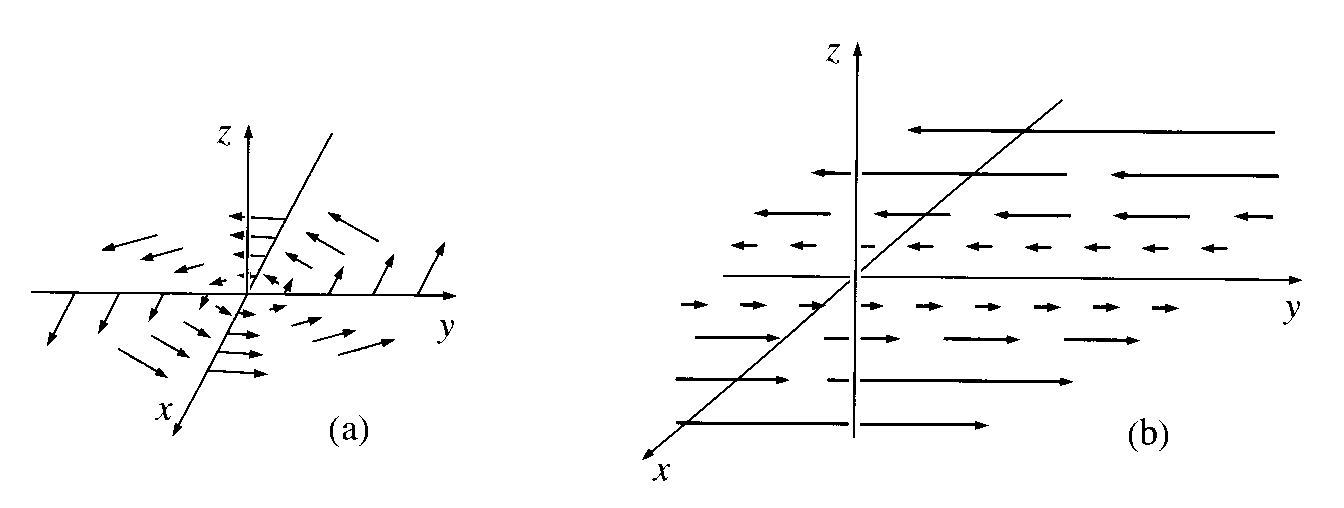
\includegraphics[width=1.0\columnwidth]{Curl.png}
\caption{เคิร์ล $\nabla\cross\vec{V}$ ภาพทั้งสองแสดงการหมุนวนของเวกเตอร์ $\vec{V}$ มีผลให้ $\nabla\cross\vec{V}$ พุ่งไปในทิศทางตามแนวแกน $z$ (ภาพจาก Griffiths 1999)}
\label{fig5}
\end{figure}

\begin{center}
\Large{\textbf{แบบฝึกหัด}}\\
\end{center}
1. จากสเกลาร์ฟังก์ชัน $V(r) = V(\sqrt{x^2 + y^2 + z^2})$ จงหาเกรเดียนท์ของสเกลาร์ฟังก์ชันนี้ \\ \underline{คำแนะนำ} ใช้กฎลูกโซ่ (chain rule) ช่วย ดังนี้\\
\begin{equation}\label{ChainRuleSpherical}
\f{\pd V(r, \theta, \phi)}{\pd x} = \f{\pd V}{\pd r}\f{\pd r}{\pd x} + \f{\pd V}{\pd \theta}\f{\pd \theta}{\pd x} + \f{\pd V}{\pd \phi}\f{\pd \phi}{\pd x} \no
\end{equation}
2. จงแสดงวิธีการพิสูจน์สมการที่ (\ref{DivFV})\\
3. สำหรับอนุภาคเคลื่อนที่เป็นวงกลมด้วยวงโคจรที่เป็นไปตามสมการ
 \begin{equation}\label{excercise2.3}
 \vec{r} = r \cos(\omega t)\i + r \sin(\omega t)\j \no
 \end{equation}
 และกำหนดให้รัศมีวงโคจร $r$ และอัตราเร็วเชิงมุม $\omega$ มีค่าคงที่\\
3.1 จงหา $\vec{r}\cdot\dot{\vec{r}}$ เมื่อ $\dot{\vec{r}} = \f{d\vec{r}}{dt} = \vec{v}$ \\
3.2 จงแสดงว่า $\ddot{\vec{r}} + \omega^2\vec{r} = 0$ เมื่อ $\ddot{\vec{r}} = \f{d\vec{v}}{dt}$\\
4. ถ้า (1) $\vec{V} = V_x(x, y)\i + V_y(x, y)\j$ และ (2) $\nabla\cross\vec{V} \neq 0$ จงแสดงว่า $\nabla\cross\vec{V}$ ตั้งฉากกับเวกเตอร์ $\vec{V}$\\

\section{ระบบพิกัด และการแปลงพิกัด}

โดยทั่วไประบบพิกัดที่เราใช้ส่วนใหญ่จะเป็นระบบพิกัดที่เรียกว่า \emph{ระบบพิกัดฉาก} (Cartesian Coordinate System) ซึ่งเป็นระบบพิกัดที่มีแกนทั้งสามตั้งฉากซึ่งกันและกัน และแต่ละแกน เราสามารถระบุพิกัดได้เป็น ($x$, $y$, $z$) และมีเวกเตอร์หน่วยเป็น $\i$, $\j$, $\k$ ตามลำดับ แต่ในบางครั้งการคำนวณหรือกระบวนการดำเนินการทางคณิตศาสตร์และฟิสิกส์ ไม่สะดวก หรือมีความซับซ้อนมากเมื่อทำการคำนวณหรือดำเนินการในระบบพิกัดฉาก และจะง่ายกว่ามากเมื่อทำการคำนวณหรือดำเนินการในระบบพิกัดอื่น ดังนั้นในหัวข้อนี้จึงได้แนะนำระบบพิกัดแบบอื่นๆ นอกเหนือจากระบบพิกัดฉาก

\subsection{ระบบพิกัดทรงกระบอก (Circular Cylinder Coordinate System)}

ในระบบพิกัดทรงกระบอกนี้ เราจะระบุพิกัดด้วย ($\rho$, $\varphi$, $z$) โดยที่ค่าของแต่ละแกนจะอยู่ในช่วงต่างๆดังนี้
\begin{equation}\label{CylinderCoorRange}
0 \leq \rho \leq \infty, \;\;\; 0 \leq \varphi \leq 2\pi, \;\;\; - \infty < z < \infty
\end{equation}

\begin{figure}%[!h]%%Figure 6
\centering
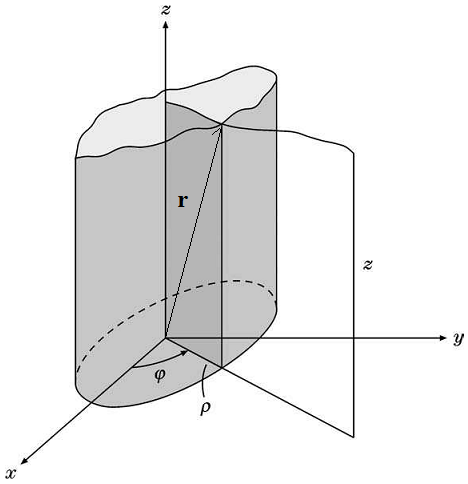
\includegraphics[width=0.75\columnwidth]{CylinderCoor.png}
\caption{ภาพแสดงระบบพิกัดทรงกระบอก ที่ระบุพิกัดด้วย ($\rho$, $\varphi$, $z$) (ตกแต่งภาพเพิ่มเติมจาก Arfken 2005)}
\label{fig6}
\end{figure}
สำหรับค่า $\rho = 0$ จะทำให้ $\varphi$ ไม่นิยาม และจากรูปที่ \ref{fig6} เราสามารถเขียนความสัมพันธ์ของระบบพิกัดทรงกระบอกกับระบบพิกัดฉากได้ดังนี้
\begin{eqnarray}\label{CylinderInCatesian}
x &=& \rho \cos (\varphi) \no \\
y &=& \rho \sin (\varphi) \\
z &=& z \no
\end{eqnarray}
นอกจากนี้ยังสามารถเขียนพิกัดทรงกระบอกในรูปของระบบพิกัดฉากได้เป็น
\begin{equation}\label{RhoInXY}
\rho = \sqrt{x^2 + y^2} = constant
\end{equation}
\begin{equation}\label{VarphiInXY}
\varphi = \tan^{-1}\l(\f{y}{x}\r)
\end{equation}
ในส่วนของเวกเตอร์ $\vec{V}$ สามารถเขียนได้เป็น
\begin{equation}\label{CylinderVecV}
\vec{V} = V_\rho\ro + V_\varphi\vp + V_z\z
\end{equation}
เวกเตอร์กระจัด $\vec{r}$ กับอนุพันธ์ขอมันสามารถเขียนได้เป็น
\begin{equation}\label{CylinderVecR}
\vec{r} = \rho\ro + z\z
\end{equation}
\begin{equation}\label{CylinderDR}
d\vec{r} = d\rho\ro + \rho d\varphi\vp + dz\z
\end{equation}
ในทำนองเดียวกัน การดำเนินการขั้นสูงสำหรับการหาอนุพันธ์สำหรับ $\nabla$ ได้เป็น
\begin{equation}\label{CylinderDel}
\nabla\;\psi(\rho, \varphi, z) = \f{\pd\psi}{\pd\rho}\ro + \f{1}{\rho}\f{\pd\psi}{\pd\varphi}\vp + \f{\pd\psi}{\pd z}\z
\end{equation}
\begin{equation}\label{CylinderDiv}
\nabla\cdot\vec{V} = \f{1}{\rho}\f{\pd}{\pd\rho}(\rho V_\rho) + \f{1}{\rho}\f{\pd V_\varphi}{\pd \varphi} + \f{\pd V_z}{\pd z}
\end{equation}
\begin{eqnarray}\label{CylinderDivSqr}
\nabla\cdot\nabla\psi &=& \nabla^2\psi \no \\
        &=& \f{1}{\rho}\f{\pd}{\pd\rho}\l(\rho\f{\pd\psi}{\pd\rho}\r) + \f{1}{\rho^2}\f{\pd^2\psi}{\pd\varphi^2} + \f{\pd^2\psi}{\pd z^2}
\end{eqnarray}
\begin{equation}\label{CylinderCurl}
\nabla\cross\vec{V} = \f{1}{\rho}\begin{vmatrix} \ro & \rho\vp & \z \\ \f{\pd}{\pd\rho} & \f{\pd}{\pd\varphi} & \f{\pd}{\pd z} \\ V_\rho & \rho V_\varphi & V_z \end{vmatrix}
\end{equation}
โดยที่เวกเตอร์หน่วยของพิกัดทรงกระบอกสัมพันธ์กับเวกเตอร์หน่วยในพิกัดฉากดังนี้
\begin{eqnarray}\label{CylinderUnitVec}
\ro &=& \cos\varphi\i + \sin\varphi\j \no \\
\vp &=& - \sin\varphi\i + \cos\varphi\j \\
\z &=& \k \no
\end{eqnarray}
ในทำนองเดียวกันเราก็สามารถเขียนเวกเตอร์หน่วยของพิกัดฉากในรูปของระบบพิกัดทรงกระบอก ได้ดังนี้
\begin{eqnarray}\label{CylinderUnitVecXYZ}
\i &=& \cos\varphi\ro - \sin\varphi\ph \no \\
\j &=& \sin\varphi\ro + \cos\varphi\ph \\
\k &=& \z \no
\end{eqnarray}

\begin{center}
\Large{\textbf{แบบฝึกหัด}}\\
\end{center}
1. จงหาผลลัพธ์ของสมการไฮโดรไดนามิกส์ของ Navier-Stokes ที่มีเทอมไม่เชิงเส้น คือ $\nabla\cross\l[\vec{v}\cross(\nabla\cross\vec{v})\r]$ เมื่อ $\vec{v}$ คือความเร็วของของไหล สำหรับของไหลที่ไหลผ่านท่อทรงกระบอกไปตามแนวแกน $z$ ตามสมการ $\vec{v} = v(\rho)\z$\\
2. จงหาองค์ประกอบของความเร็วและความเร่งของอนุภาคที่กำลังเคลื่อนที่ในระบบพิกัดทรงกระบอก เมื่อเวกเตอร์ตำแหน่งของอนุภาคที่ขึ้นกับเวลาเป็นไปตามสมการ
\begin{eqnarray}\label{CylinderProblem2}
\vec{r}(t) &=& \rho(t)\ro(t) + z(t)\z \no \\
        &=& \l[\cos \varphi(t)\hat{x} + \sin \varphi(t)\hat{y}\r]\rho(t) + z(t)\z \no
\end{eqnarray}
เมื่อ $\dot{\rho} = d\rho/dt$, $\ddot{\rho} = d^2\rho/dt^2$\\
3. จงแก้สมการลาปลาซ $\nabla^2\psi = 0$ ในระบบพิกัดทรงกระบอกเมื่อ $\psi = \psi(\rho)$

\subsection{ระบบพิกัดเชิงขั้วทรงกลม (Spherical Polar Coordinate System)}

ในระบบพิกัดเชิงขั้วทรงกลมจะระบุตำแหน่งด้วยพิกัด ($r$, $\theta$, $\phi$) ซึ่งแสดงให้เห็นดังรูปที่ \ref{fig7}

\begin{figure}[!h]%%Figure 7
\centering
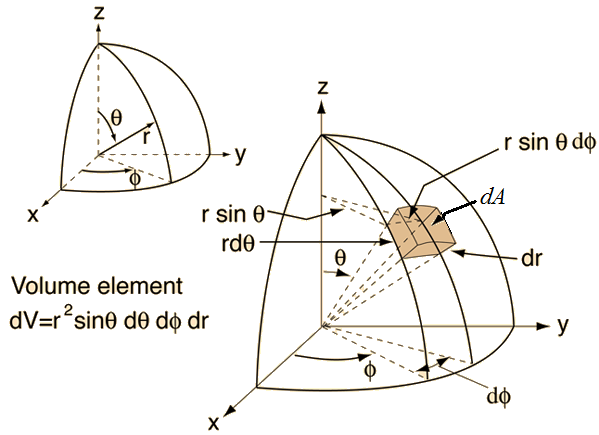
\includegraphics[width=0.75\columnwidth]{sphcoordel.png}
\caption{ภาพแสดงระบบพิกัดเชิงขั้วทรงกลม ที่ระบุพิกัดด้วย ($r$, $\theta$, $\phi$) (ตกแต่งภาพเพิ่มเติมจากอินเตอร์เนต)}
\label{fig7}
\end{figure}
และพิกัดเหล่านี้สัมพันธ์กับระบบพิกัดฉาก โดยที่ขนาดของเวกเตอร์ตำแหน่ง $\vec{r} $ สามารถเขียนได้เป็น
\begin{equation}\label{SphereCoorR}
r = \sqrt{x^2 + y^2 + z^2} = constant
\end{equation}
มุม $\theta$ ที่ทำกับแกน $z$ หาได้จากความสัมพันธ์
\begin{equation}\label{SphereCoorTheta}
\theta = \cos^{-1}\l(\f{z}{r}\r) = constant
\end{equation}
และมุม $\phi$ บนระนาบ $xy$ สามารถหาได้จากสมการ
\begin{equation}\label{SphereCoorPhi}
\phi = \tan^{-1}\l(\f{y}{x}\r) = constant
\end{equation}
ดังนั้น เราจึงสามารถเขียนต่อมาได้ว่า
\begin{eqnarray}\label{SphereCoorXYZ}
x &=& r \sin\theta\cos\phi \no \\
y &=& r \sin\theta\sin\phi \\
z &=& r \cos\theta \no
\end{eqnarray}
โดยมีเวกเตอร์ตำแหน่ง
\begin{eqnarray}\label{SphereCoorVecR}
\vec{r} &=& r\rh \no \\
        &=& x\i + y\j + z\k \no \\
        &=& r\sin\theta\cos\phi\i + r \sin\theta\sin\phi\j + r \cos\theta\k
\end{eqnarray}
และอนุพันธ์ของเวกเตอร์ตำแหน่งเขียนได้เป็น
\begin{equation}\label{SphereCoordR}
d\vec{r} = dr\rh + rd\theta\tt + r \sin\theta d\phi\ph
\end{equation}
นอกจากนี้ยังมีส่วนของพื้นที่น้อยๆ (area element, $dA$) ที่มีรัศมี $r$ คงที่ และส่วนของมุมตัน (solid angle, $d\Omega$) ที่รองรับพื้นที่ $dA$ นี้ สามารถเขียนได้ดังนี้ ตามลำดับ
\begin{equation}\label{SphereCoordA}
dA = d\sigma_{\theta\phi} = r^2 \sin\theta d\theta d\phi
\end{equation}
\begin{equation}\label{SphereCoordOmega}
d\Omega = \f{dA}{r^2} = \sin\theta d\theta d\phi
\end{equation}
และการอินทิเกรตตลอดทั้งพื้นผิวทรงกลม จะได้ว่า
\begin{equation}\label{SphereCoorIntdOmega}
\int d\Omega = 4\pi
\end{equation}
นอกจากนี้ยังมีส่วนของปริมาตรน้อยๆ (volume element) ของพิกัดเชิงขั้วทรงกลมเขียนได้เป็น
\begin{equation}\label{ShereCoorVolElement}
d\tau = r^2 dr \sin\theta d\theta d\phi = r^2 dr d\Omega
\end{equation}
ในส่วนของเวกเตอร์หน่วยในระบบพิกัดเชิงขั้วทรงกลม ($\rh$, $\tt$, $\ph$) สามารถเขียนความสัมพันธ์กับระบบพิกัดฉาก ได้ดังนี้
\begin{eqnarray}\label{SphereCoorUnitVec}
\rh &=& \sin\theta\cos\phi\i + \sin\theta\sin\phi\j + \cos\theta\k \no \\
\tt &=& \cos\theta\cos\phi\i + \cos\theta\sin\phi\j - \sin\theta\k = \f{\pd\rh}{\pd\theta} \\
\ph &=& - \sin\phi\i + \cos\phi\j = \f{1}{\sin\theta}\f{\pd\rh}{\pd\phi} \no
\end{eqnarray}
และในทางกลับกันเราก็จะได้
\begin{eqnarray}\label{SphereCoorUnitVecXYZ}
\i &=& \sin\theta\cos\phi\rh + \cos\theta\cos\phi\tt - \sin\phi\ph \no \\
\j &=& \sin\theta\sin\phi\rh + \cos\theta\sin\phi\tt + \cos\phi\ph \\
\k &=& \cos\theta\rh - \sin\theta\tt \no
\end{eqnarray}

ส่วนของการดำเนินการขั้นสูงเกี่ยวกับ $\nabla$ สามารถเขียนได้ดังนี้
\begin{equation}\label{SphereCoorGrad}
\nabla\psi = \f{\pd\psi}{\pd r}\rh + \f{1}{r}\f{\pd\psi}{\pd\theta}\tt + \f{1}{r \sin\theta}\f{\pd\psi}{\pd\phi}\ph
\end{equation}
\begin{equation}\label{SphereCoorDiv}
\nabla\cdot\vec{V} = \f{1}{r^2 \sin\theta}\l[\sin\theta\f{\pd}{\pd r}\l(r^2V_r\r) + r\f{\pd}{\pd\theta}\l(\sin\theta V_\theta\r) + r\f{\pd V_\phi}{\pd\phi}\r]
\end{equation}
\begin{eqnarray}\label{SphereCoorLaplace}
\nabla\cdot\nabla\psi &=& \nabla^2\psi \no \\
        &=& \f{1}{r^2 \sin\theta}\Bigg[\sin\theta\f{\pd}{\pd r}\l(r^2\f{\pd\psi}{\pd r}\r) + \f{\pd}{\pd\theta}\l(\sin\theta\f{\pd\psi}{\pd\theta}\r) \no \\
        & & +\;\f{1}{\sin\theta}\f{\pd^2\psi}{\pd\phi^2}\Bigg]
\end{eqnarray}
\begin{equation}\label{SphereCoorCurl}
\nabla\cross\vec{V} = \f{1}{r^2 \sin\theta}\begin{vmatrix} \rh & r\tt & r \sin\theta\ph \\ \f{\pd}{\pd r} & \f{\pd}{\pd\theta} & \f{\pd}{\pd\phi} \\ V_r & rV_\theta & r \sin\theta V_\phi \end{vmatrix}
\end{equation}

\begin{figure}[!h]%%Figure 7
\centering
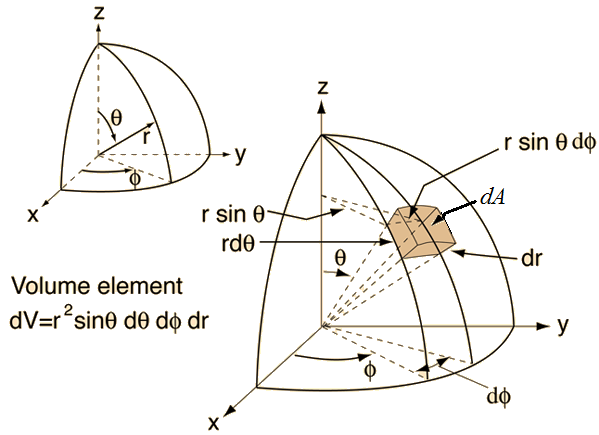
\includegraphics[width=0.75\columnwidth]{sphcoordel.png}
\caption{ภาพแสดงระบบพิกัดเชิงขั้วทรงกลม ที่ระบุพิกัดด้วย ($r$, $\theta$, $\phi$) (ตกแต่งภาพเพิ่มเติมจากอินเตอร์เนต)}
\label{fig7}
\end{figure}

\begin{figure}[!h]%%Figure 7
\centering
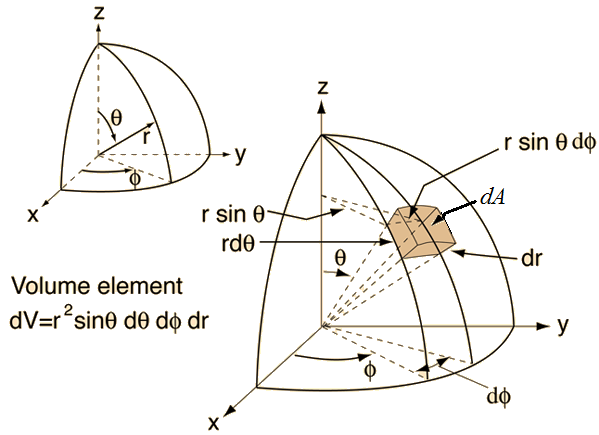
\includegraphics[width=0.75\columnwidth]{sphcoordel.png}
\caption{ภาพแสดงระบบพิกัดเชิงขั้วทรงกลม ที่ระบุพิกัดด้วย ($r$, $\theta$, $\phi$) (ตกแต่งภาพเพิ่มเติมจากอินเตอร์เนต)}
\label{fig7}
\end{figure}

\begin{figure}[!h]%%Figure 7
\centering
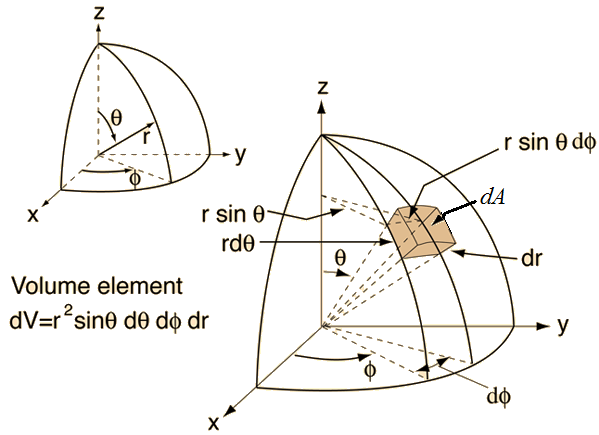
\includegraphics[width=0.75\columnwidth]{sphcoordel.png}
\caption{ภาพแสดงระบบพิกัดเชิงขั้วทรงกลม ที่ระบุพิกัดด้วย ($r$, $\theta$, $\phi$) (ตกแต่งภาพเพิ่มเติมจากอินเตอร์เนต)}
\label{fig7}
\end{figure}

\begin{figure}[!h]%%Figure 7
\centering
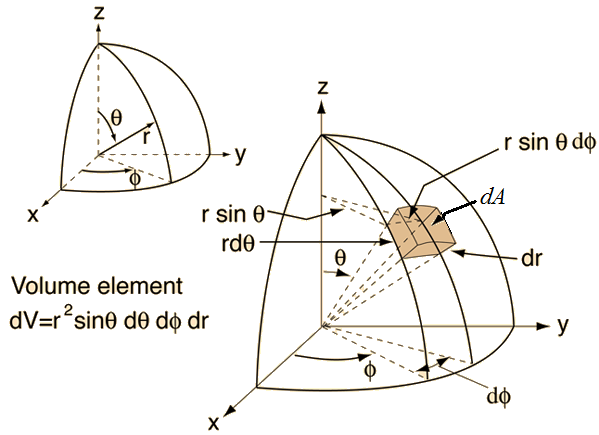
\includegraphics[width=0.75\columnwidth]{sphcoordel.png}
\caption{ภาพแสดงระบบพิกัดเชิงขั้วทรงกลม ที่ระบุพิกัดด้วย ($r$, $\theta$, $\phi$) (ตกแต่งภาพเพิ่มเติมจากอินเตอร์เนต)}
\label{fig7}
\end{figure}

\begin{figure}[!h]%%Figure 7
\centering
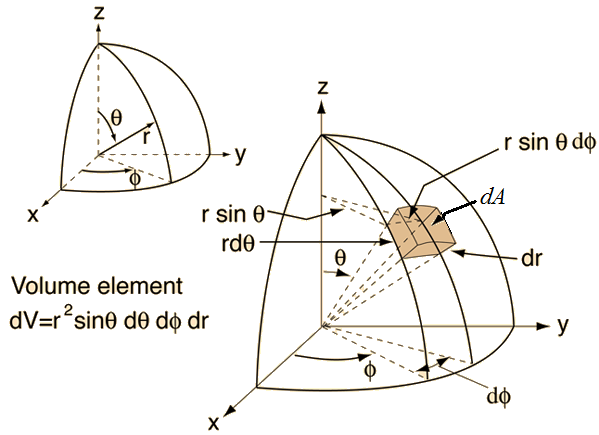
\includegraphics[width=0.75\columnwidth]{sphcoordel.png}
\caption{ภาพแสดงระบบพิกัดเชิงขั้วทรงกลม ที่ระบุพิกัดด้วย ($r$, $\theta$, $\phi$) (ตกแต่งภาพเพิ่มเติมจากอินเตอร์เนต)}
\label{fig7}
\end{figure}

\begin{figure}[!h]%%Figure 7
\centering
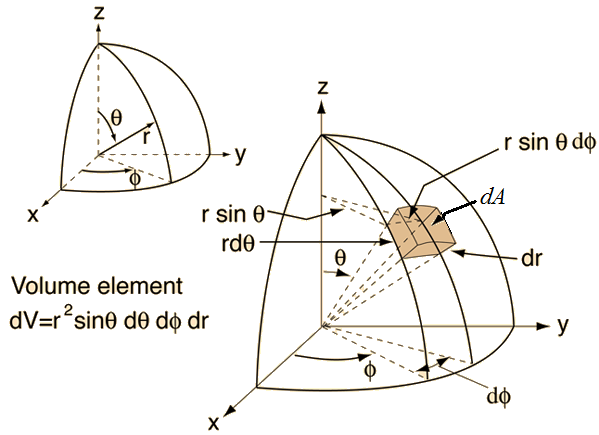
\includegraphics[width=0.75\columnwidth]{sphcoordel.png}
\caption{ภาพแสดงระบบพิกัดเชิงขั้วทรงกลม ที่ระบุพิกัดด้วย ($r$, $\theta$, $\phi$) (ตกแต่งภาพเพิ่มเติมจากอินเตอร์เนต)}
\label{fig7}
\end{figure}

\begin{figure}[!h]%%Figure 7
\centering
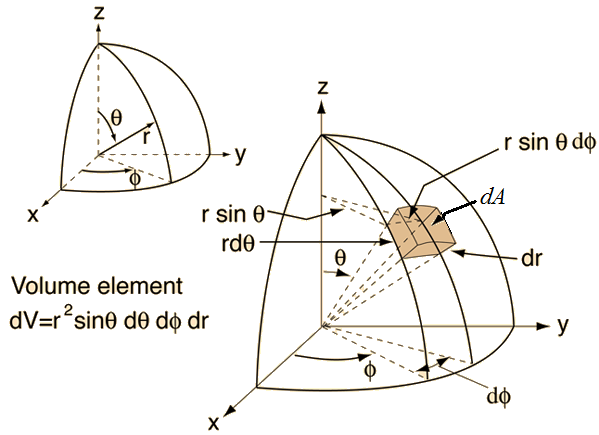
\includegraphics[width=0.75\columnwidth]{sphcoordel.png}
\caption{ภาพแสดงระบบพิกัดเชิงขั้วทรงกลม ที่ระบุพิกัดด้วย ($r$, $\theta$, $\phi$) (ตกแต่งภาพเพิ่มเติมจากอินเตอร์เนต)}
\label{fig7}
\end{figure}

\begin{figure}[!h]%%Figure 7
\centering
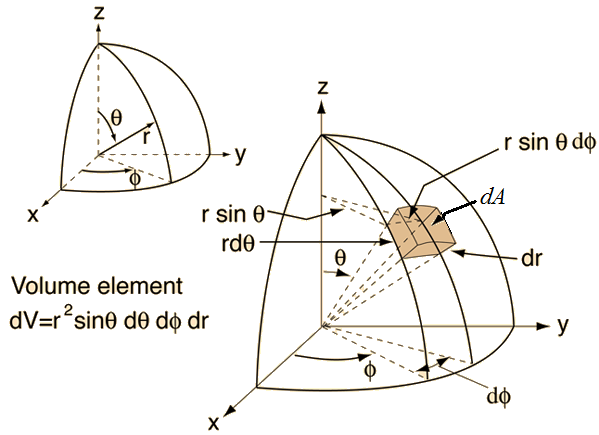
\includegraphics[width=0.75\columnwidth]{sphcoordel.png}
\caption{ภาพแสดงระบบพิกัดเชิงขั้วทรงกลม ที่ระบุพิกัดด้วย ($r$, $\theta$, $\phi$) (ตกแต่งภาพเพิ่มเติมจากอินเตอร์เนต)}
\label{fig7}
\end{figure}

\begin{figure}[!h]%%Figure 7
\centering
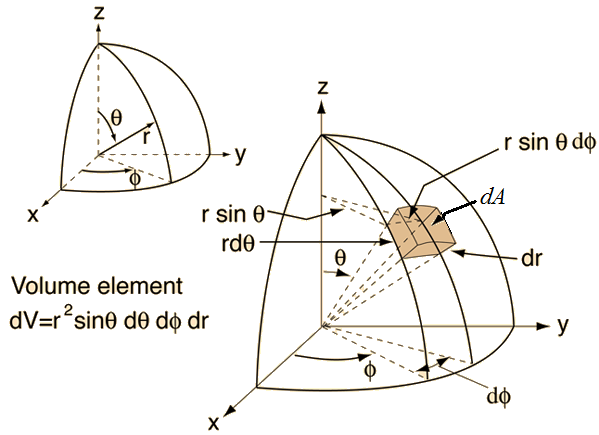
\includegraphics[width=0.75\columnwidth]{sphcoordel.png}
\caption{ภาพแสดงระบบพิกัดเชิงขั้วทรงกลม ที่ระบุพิกัดด้วย ($r$, $\theta$, $\phi$) (ตกแต่งภาพเพิ่มเติมจากอินเตอร์เนต)}
\label{fig7}
\end{figure}

\begin{figure}[!h]%%Figure 7
\centering
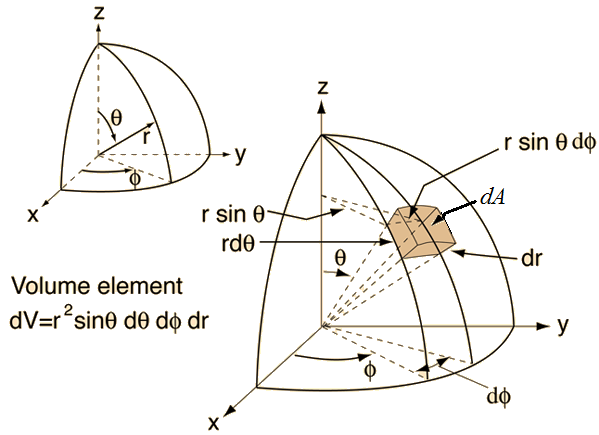
\includegraphics[width=0.75\columnwidth]{sphcoordel.png}
\caption{ภาพแสดงระบบพิกัดเชิงขั้วทรงกลม ที่ระบุพิกัดด้วย ($r$, $\theta$, $\phi$) (ตกแต่งภาพเพิ่มเติมจากอินเตอร์เนต)}
\label{fig7}
\end{figure}

\begin{figure}[!h]%%Figure 7
\centering
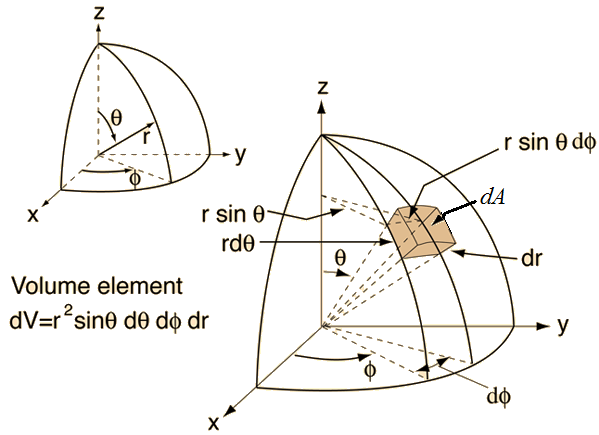
\includegraphics[width=0.75\columnwidth]{sphcoordel.png}
\caption{ภาพแสดงระบบพิกัดเชิงขั้วทรงกลม ที่ระบุพิกัดด้วย ($r$, $\theta$, $\phi$) (ตกแต่งภาพเพิ่มเติมจากอินเตอร์เนต)}
\label{fig7}
\end{figure}

\begin{center}
\Large{\textbf{แบบฝึกหัด}}\\
\end{center}
1. จากสมการ
\begin{equation}\label{SphereCoorProblem1}
\mu_0\vec{J} = \nabla\cross[\nabla\cross A_\phi(r, \theta)\ph
\end{equation}
จงหาผลลัพธ์ในระบบพิกัดเชิงขั้วทรงกลม \underline{ข้อแนะนำ} ให้ทำการหาเคิร์ลในระบบพิกัดเชิงขั้วทรงกลมสองครั้ง\\
2. จงหาองค์ประกอบของความเร็วและความเร่งของอนุภาคที่กำลังเคลื่อนที่ในระบบพิกัดเชิงขั้วทรงกลม โดยเวกเตอร์ตำแหน่งเขียนได้เป็น
\begin{eqnarray}\label{SphereCoorProblem2}
\vec{r}(t) &=& r(t)\rh(t) \no \\
        &=& r(t)\l[\sin\theta(t)\cos\phi(t)\i + \sin\theta(t)\sin\phi(t)\j + \cos\theta(t)\k\r] \no
\end{eqnarray}
โดยที่ $\dot{r} = dr/dt$, $\dot{\theta} = d\theta/dt$, $\dot{\phi} = d\phi/dt$\\

\section{เทนเซอร์เบื้องต้น}

เทนเซอร์ (tensor) เป็นปริมาณทางฟิสิกส์ชนิดหนึ่ง ซึ่งมีความสำคัญทางฟิสิกส์เป็นอย่างยิ่ง ปริมาณสเกลาร์ และเวกเตอร์ ก็เป็นกรณีเฉพาะของเทนเซอร์เช่นเดียวกัน นั่นคือ สเกลาร์เป็น \emph{เทนเซอร์แรงค์ศูนย์} (tensor of rank 0) ส่วนเวกเตอร์เป็น \emph{เทนเซอร์แรงค์หนึ่ง} (tensor of rank 1) โดยในระบบพิกัดฉากสามมิติ เวกเตอร์มีองค์ประกอบทั้งหมด $3^1 = 3$ ตัว และถ้าเป็นเทนเซอร์แรงค์ $n$ จะมีองค์ประกอบทั้งหมด $3^n$ ตัว\footnote{ในระบบพิกัด $N$ มิติ สำหรับเทนเซอร์แรงค์ $n$ จะมีองค์ประกอบทั้งหมด $N^n$ ตัว}

\subsection{การแปลงเทนเซอร์ (Tensor Transformation)}
พิจารณาการแปลงของเทนเซอร์แรงค์หนึ่ง หรือการแปลงเวกเตอร์ (vector transformation) เราสามารถเขียนได้เป็น
\begin{equation}\label{VecTransformD}
A'_i = \sum_j a_{ij}A_j
\end{equation}
เมื่อ $a_{ij}$ เป็น $\cos$ ของมุมระหว่างแกน $x'_i$ กับแกน $x_j$ หรือเขียนในรูปของอนุพันธ์ได้เป็น
\begin{equation}\label{VecTransformDiff}
dx'_i = \sum_j \f{\pd x'_i}{\pd x_j}dx_j
\end{equation}
โดยที่ $a_{ij} = \pd x'_i/\pd x_j$ ดังนั้นเมื่อเราใช้นิยามของ $a_{ij}$ ดังนี้แล้ว เราจึงสามารถเขียนการแปลงเวกเตอร์จากสมการ (\ref{VecTransformD}) ได้ใหม่เป็น
\begin{equation}\label{VecTransformConV}
A'^i = \sum_j \f{\pd x'_i}{\pd x_j}A^j
\end{equation}
และเรียกว่าเป็น \emph{คอนทราวาเรียนเวกเตอร์} (contravariant vector) ซึ่งเป็นการเขียนอินเดกซ์ของเวกเตอร์เป็นตัวอินเดกซ์บน (superscript index) แลละในกรณีนี้สำหรับเวกเตอร์ในระบบพิกัดฉาก เราจะกำหนดให้ $x^i = x_i$ นับตั้งแต่นี้ไป นอกจากนี้ยังมีกรณีที่เขียนอินเดกซ์ของเวกเตอร์เป็นตัวอินเดกซ์ล่าง (subscript index) ซึ่งเขียนได้เป็น
\begin{equation}\label{VecTransformCoV}
A'_i = \sum_j \f{\pd x^j}{\pd x'^i}A_j
\end{equation}
และเรียกว่า \emph{โควาเรียนท์เวกเตอร์} (covariant vector) และในเฉพาะระบบพิกัดฉากเท่านั้น เราจะได้ว่า
\begin{equation}\label{TransformCoeff}
\f{\pd x^j}{\pd x'^i} = \f{\pd x'^i}{\pd x^j} = a_{ij}
\end{equation}

สำหรับเทนเซอร์ตั้งแต่แรงค์สอง (tensor of rank 2) ขึ้นไป เราสามารถที่จะเขียนอินเดกซ์ได้ทั้งแบบโควาเรียนท์, คอนทราวาเรียนท์ หรือแบบผสมก็ได้ ดังนี้
\begin{eqnarray}\label{TensorTransformR2}
A'^{ij} &=& \sum_{kl}\f{\pd x'^i}{\pd x^k}\f{\pd x'^j}{\pd x^l}A^{kl} \no \\
B'^i_j &=& \sum_{kl}\f{\pd x'^i}{\pd x^k}\f{\pd x^l}{\pd x'^j}B^k_l \\
C'_{ij} &=& \sum_{kl}\f{\pd x^k}{\pd x'^i}\f{\pd x^l}{\pd x'^j}C_{kl} \no
\end{eqnarray}
ดังนั้น เราสามารถสรุปได้ว่า \\
\emph{เทนเซอร์เป็นปริมาณที่องค์ประกอบของมันมีการจัดการด้วยอินเดกซ์หนึ่งตัวหรือมากกว่านั้น โดยจำนวนของอินเดกซ์เราเรียกว่าแรงค์ของเทนเซอร์ (rank of tensor) เช่น เทนเซอร์แรงค์ศูนย์ (สเกลาร์) $A$, เทนเซอร์แรงค์หนึ่ง (เวกเตอร์) $A^i$, เทนเซอร์แรงค์สอง $A^{ij}$ หรือ $A^i_j$ หรือ $A_{ij}$ เป็นต้น}

\subsection{สมบัติของเทนเซอร์ (Tensor Properties)}

สำหรับการบวก การลบ ของเทนเซอร์เราสามารถเขียนได้เป็น
\begin{equation}\label{TensorPropAdd}
A^{ij} + B^{ij} = C^{ij}
\end{equation}
นอกจากนี้ยังมีสิ่งที่เรียกว่า ธรรมเนียมปฏิบัติการบวก (summation convention) ซึ่งหมายถึงการบวกเทนเซอร์โดยไม่เขียนเครื่องหมาย การบวก $\sum$ และถือว่ามีการบวกกัน กรณีที่มีอินเดกซ์ซ้ำกัน ตัวอย่างเช่น จากการแปลงเทนเซอร์ ในสมการ (\ref{TensorTransformR2}) เราสามารถเขียนได้เป็น
\begin{equation}\label{SummationConvention}
B'^i_j = \f{\pd x'^i}{\pd x^k}\f{\pd x^l}{\pd x'^j}B^k_l
\end{equation}
จะเห็นว่ามีการบวกกันผ่านอินเดกซ์ที่ซ้ำกันทางด้านขวา คือ อินเดกซ์ $k$ และ $l$ และนี่เป็นสิ่งที่เรียกว่า \emph{ธรรมเนียมปฏิบัติการบวกของไอน์สไตน์} (Einstein's summation convention) หรือเรียกสั้นๆว่า \emph{ธรรมเนียมปฏิบัติการบวก} ในการนี้เราสามารถโยงเข้ากับโครนเนคเกอร์เดลต้าฟังก์ชัน $\delta^k_l$ ได้ดังนี้
\begin{equation}\label{KroneckerDelta}
\delta^k_l\f{\pd x'^i}{\pd x^k}\f{\pd x^l}{\pd x'^j} = \f{\pd x'^i}{\pd x^k}\f{\pd x^k}{\pd x'^j}
\end{equation}
และจากนิยามของโครนเนคเกอร์เดลต้า เราจะได้ว่า
\begin{equation}\label{Contraction}
\f{\pd x'^i}{\pd x^k}\f{\pd x^k}{\pd x'^j} = \f{\pd x'^i}{\pd x'^j} = \delta'^i_j
\end{equation}
ดังนั้น สำหรับการแปลงของโครนเนคเกอร์เดลต้าฟังก์ชัน สามารถเขียนได้เป็น
\begin{equation}\label{KroneckerDeltaTransform}
\delta'^i_j = \f{\pd x'^i}{\pd x^k}\f{\pd x^l}{\pd x'^j}\delta^k_l
\end{equation}
กรณีที่อินเดกซ์ซ้ำกันนอกจากจะหมายถึงการบวกกันแล้ว เรายังสามารถทำการยุบอินเดกซ์ (index contraction) ได้อีกด้วย โดยผ่านการใช้โครนเนคเกอร์เดลต้าฟังก์ชัน
\begin{equation}\label{ContractionTensorR2}
B'^i_i = \f{\pd x'^i}{\pd x^k}\f{\pd x^l}{\pd x'^i}B^k_l = \f{\pd x^l}{\pd x^k}B^k_l
\end{equation}
ในกรณีนี้ ส่วนสุดท้ายจะมีการลดรูปของอินเดกซ์และเขียนในรูปโครนเนคเกอร์เดลต้า คือ $\delta^i_i = 1$ แต่ละไว้ในฐานที่เข้าใจ หรือสามารถเขียนให้ชัดเจนได้เป็น
\begin{equation}\label{ContractionTensorDelta}
B'^i_i = \delta^i_i\delta^l_kB^k_l = \delta^l_kB^k_l = B^k_k
\end{equation}
หรือสามารถเขียนพิจารณาได้ง่ายๆ จากเทนเซอร์แรงค์ $n$ ดังนี้
\begin{equation}\label{ContractionTensorRn}
\tensor{A}{^{ijklm}_{klmst}^{...tuv}_{...vw}} = \tensor{A}{^{ij}_{s}^{..u}_{...w}}
\end{equation}
นั่นคือ มีการใช้ธรรมเนียมปฏิบัติการบวก หรือใส่โครนเนคเกอร์เดลต้าฟังก์ชันเข้าไปสำหรับอินเดกซ์ที่ซ้ำกัน คือ $\delta^k_k = 1$ นั่นเอง ซึ่งจากสมการข้างบนจะเห็นว่ามีการยุบอินเดกซ์ (index contraction) เนื่องจากการใส่โครนเนคเกอร์เดลต้าฟังก์ชันเข้าไปสำหรับอินเดกซ์ $k$, $l$, $m$, $t$, และ $v$ จึงทำให้เกิดการลดรูปของเทนเซอร์จากเทนเซอร์แรงค์ $n$ เป็นเทนเซอร์แรงค์ $n - 10$ เพราะอินเดกซ์มีการยุบหายไป 10 ตัวนั่นเอง

นอกจากนี้การเขียนสลับอินเดกซ์จะสามารถเขียนสลับได้และจะให้ค่าเหมือนเดิมหรือต่างออกไป ดังนี้
\begin{equation}\label{SymmetryTensor}
A^{mn} = A^{nm}
\end{equation}
ซึ่งเราเรียกว่าเป็น \emph{เทนเซอร์แบบสมมาตร} (symmetric tensor) และอีกรูปแบบหนึ่ง
\begin{equation}\label{AntisymmetryTensor}
A^{mn} = - A^{nm}
\end{equation}
ซึ่งเรียกว่า \emph{เทนเซอร์แบบอสมมาตร} (antisymmetric tensor) และเราสามารถเขียนเทนเซอร์แรงค์สองในแบบผสมทั้งกรณีสมมาตรและอสมมาตรได้ดังนี้
\begin{equation}\label{MixedSymTensor}
A^{mn} = \f{1}{2}\l(A^{mn} + A^{nm}\r) + \f{1}{2}\l(A^{mn} - A^{nm}\r)
\end{equation}
โดยที่ในวงเล็บแรกทางขวามือเป็นส่วนของเทนเซอร์แบบสมมาตร และในวงเล็บที่สองของทางขวามือเป็นส่วนของเทนเซอร์แบบอสมมาตร
